\documentclass[12pt]{article}
\usepackage[english]{babel}
\usepackage{graphicx}
\usepackage{times}
\usepackage{wrapfig}
\newcommand{\BibTeX}{{\sc Bib}\TeX}
\begin{document}
\title{Algorithm for long multiplication}
\author{Author:Shefali Garg\\11678\\CSE}
\date{3 Sept 2012}
\maketitle
\tableofcontents
\section{Problem Statement}


Write an algorithm to do long integer multiplication which was developed by developed by Leslie
Lamport\cite{lamport94},i.e., an algorithm to multiply two integers given as a list of their digits.

\section{Algorithm}
\begin{wrapfigure}{r}{0.1\textwidth}
  \vspace{-2pt}
  \begin{center}
    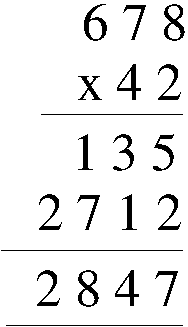
\includegraphics[width=0.1\textwidth]{mult2}
  \end{center}
  \vspace{-10pt}
  \caption{example}
  \vspace{-20pt}
\end{wrapfigure}
Given two integers,assign one with greater number of digits as primary number and other one as seconday number.If both have equal number of digits,consider any of them to be primary number.
Then take the last digit of the secondary number and do simple multiplication of that digit with the primary number.Write the obtained result just below the secondary number.Let us take an example from Donald Knuth's algo system\cite{knuth79} 
Then take the second last digit of the secondary number and do simple multiplication with the primary number.Multiply the result obtained with 10 and write it just below the number obtained in the previous step.Similarly,multiply all the digits of the secondary number with the primary number and write the result by multiplying it with power of 10,i.e.,10,100 and so on.Then do simple addition on all the numbers got above.The result is the required answer.For example-multiplication of 678 and 42 is shown in adjacent figure.
\newline
\begin{figure}[h!]
  \caption{flowchart}
  \centering
    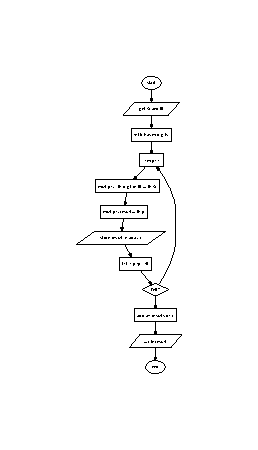
\includegraphics[width=0.5\textwidth]{flow}
\end{figure}
\section{Analysing time complexity}
Let the two given numbers are of size n.In this algorithm,each digit of the secondary number is multiplied with each digit of the primary number once.So,the total number of steps taken here is $n^2$ ,i.e.,of O($n^2$).The addition of the two n digit numbers has the time complexity of order n.Here,the addition of n numbers is done so the time complexity of addition process is of order $n^2$.So,the overall time complexity of the algorithm is O($n^2$) and the time take by the algorithm is propotional to $n^2$.There is a detailed explanation of complexity in Companion\cite{goossens93} and Rahtz's\cite{rahtz89}
\bibliographystyle{plain}
\bibliography{mult}
\end{document}
